\documentclass[main]{subfiles}


\title[AutoML: Introduction]{AutoML Motivation}
\subtitle{The AutoML MOOC Team}
\author[Marius Lindauer]{Marius Lindauer}
\date{}

\titlebackground*{images/AutoML_AutoDL}

%\institute{}
%\date{}

\begin{document}
	
	\maketitle
	

%----------------------------------------------------------------------
%----------------------------------------------------------------------
\begin{frame}[c]{The Team}

\begin{itemize}
    \item Team of researchers working on AutoML for many years; some of them for more than a decade
    \item Diverse backgrounds on different topics of AutoML
    \item Heavy focus on Germany/Europe
\end{itemize}

\end{frame}
%-----------------------------------------------------------------------
%----------------------------------------------------------------------
\begin{frame}[c]{Marius Lindauer}

\begin{columns}

\column{0.3\textwidth}

\centering
\includegraphics[width=0.9\textwidth]{team/Marius Lindauer_05_potr.jpg}


\column{0.7\textwidth}

\begin{itemize}
    \item \textit{Affiliation}: Leibniz University Hannover
    \item \textit{Position}: Full professor of machine learning
    \item \textit{Research foci}: Human-centered AutoML, Automated Reinforcement Learning, Green AutoML
    \item \textit{Highlights}: ERC Starting Grant on ixAutoML, co-author of SMAC, Auto-PyTorch and Auto-Sklearn
\end{itemize}
    
\end{columns}

\end{frame}
%-----------------------------------------------------------------------
%----------------------------------------------------------------------
\begin{frame}[c]{Marcel Wever}

\begin{columns}

\column{0.3\textwidth}

\centering

\includegraphics[width=0.9\textwidth]{01_AutoML/team/Marcel_Wever_001.jpg}


\column{0.7\textwidth}

\begin{itemize}
    \item \textit{Affiliation}: Leibniz University Hannover
    \item \textit{Position}: Postdoctoral Researcher, Research Group Leader
    \item \textit{Research foci}: Human-centered AutoML, Green AutoML, Multi-Label Classification
    \item \textit{Highlights}: core dev of OpenML, SMAC, and DeepCAVE, co-author of ML-Plan and Na{\"i}ve AutoML
\end{itemize}
    
\end{columns}

\end{frame}
%-----------------------------------------------------------------------
%----------------------------------------------------------------------
\begin{frame}[c]{Katharina Eggensperger}

\begin{columns}

\column{0.3\textwidth}

\centering
\includegraphics[width=0.9\textwidth]{01_AutoML/team/katharina_eggensperger.JPG}


\column{0.7\textwidth}

\begin{itemize}
    \item \textit{Affiliation}: Lamarr Institute and TU Dortmund University
    \item \textit{Position}: Professor for Machine Learning and Artificial Intelligence
    \item \textit{Research foci}: foundation models for tabular data, meta-science, and ML in science.
    \item \textit{Highlights}: co-core dev of auto-sklearn, AutoML competition winner, co-author of TabPFNv1, co-organizer of AutoML workshops, conferences, and summer schools.
\end{itemize}
    
\end{columns}

\end{frame}
%-----------------------------------------------------------------------
%----------------------------------------------------------------------
\begin{frame}[c]{Lars Kotthoff}

\begin{columns}

\column{0.3\textwidth}

\centering
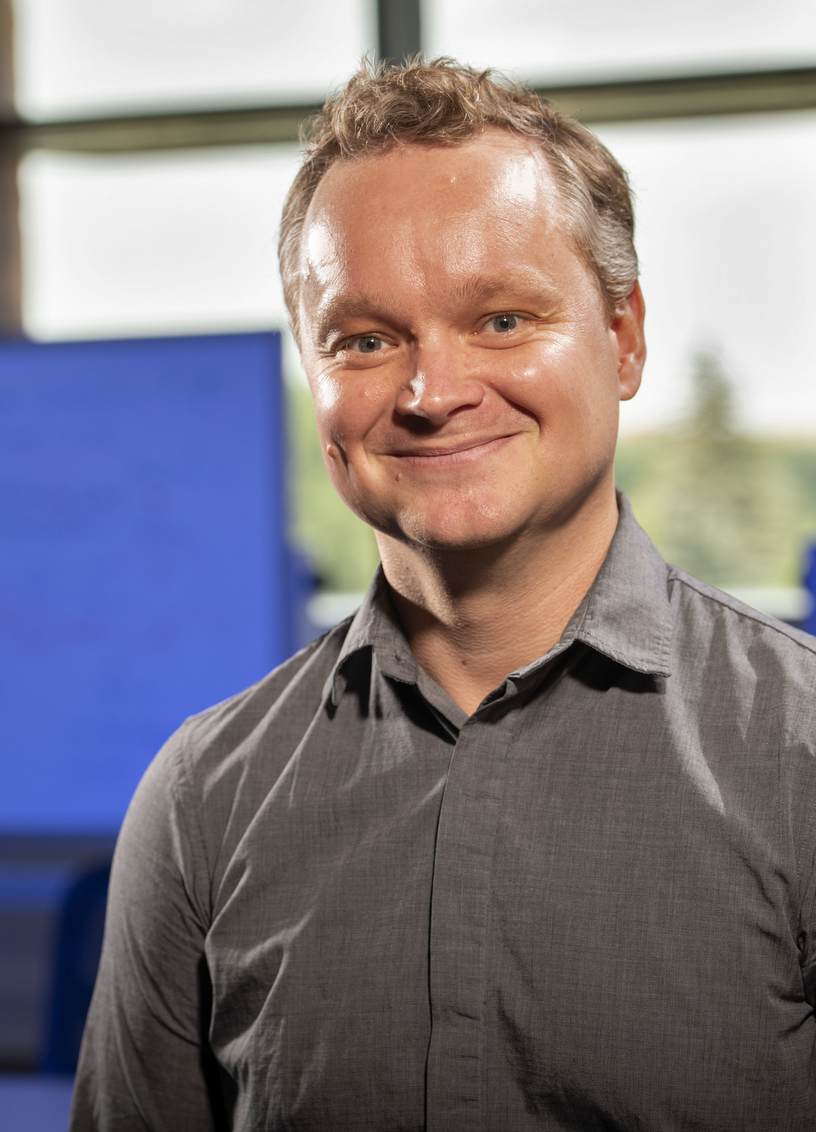
\includegraphics[width=0.9\textwidth]{team/larsko.jpg}


\column{0.7\textwidth}

\begin{itemize}
    \item \textit{Affiliation}: University of St Andrews
    \item \textit{Position}: Professor of AI
    \item \textit{Research foci}: (Auto-)ML, applications of ML in other areas, LLMs for code generation for ML and GOFAI
    \item \textit{Highlights}: Co-author of the first AutoML book, contributor to various ML software packages, wrote his own email client
\end{itemize}
    
\end{columns}

\end{frame}
%-----------------------------------------------------------------------
%----------------------------------------------------------------------
\begin{frame}[c]{Bernd Bischl}

\begin{columns}

\column{0.3\textwidth}

\centering
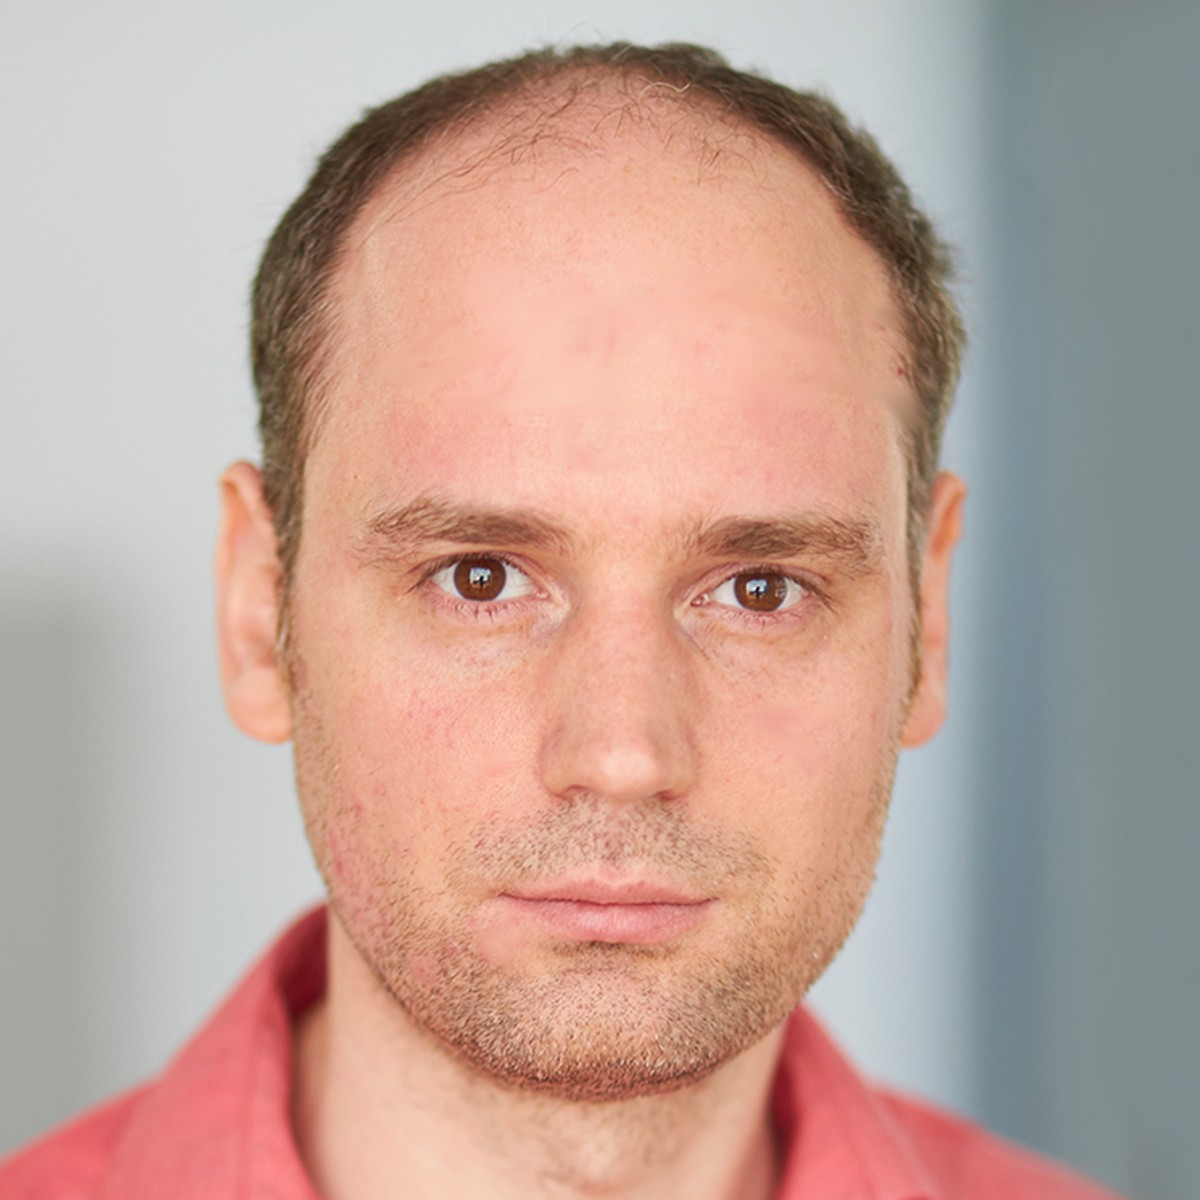
\includegraphics[width=0.9\textwidth]{team/bernd-bischl.jpg}


\column{0.7\textwidth}

\begin{itemize}
    \item \textit{Affiliation}: LMU Munich, Munich Center for ML
    \item \textit{Position}: Professor for Statistical Learning and Data Science, Co-Director of MCML
    \item \textit{Research foci}: AutoML, BO, Interpretability, Benchmarking, combos of these 
    \item \textit{Highlights}: Core OpenML, invented mlr, wrote large BO package, some papers
\end{itemize}
    
\end{columns}

\end{frame}
%-----------------------------------------------------------------------
%----------------------------------------------------------------------
\begin{frame}[c]{André Biedenkapp}

\begin{columns}

\column{0.3\textwidth}

\centering
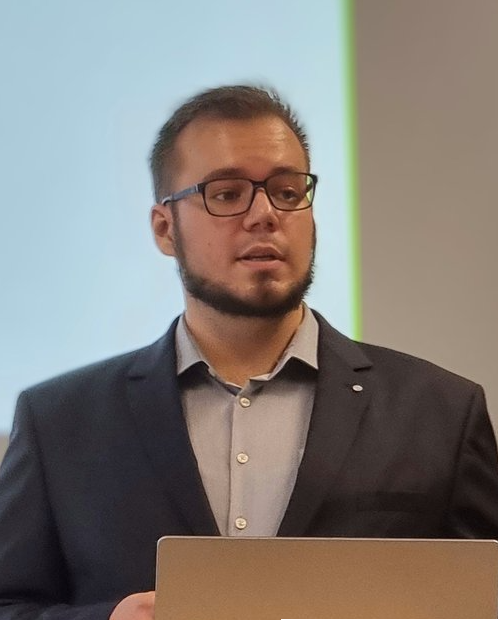
\includegraphics[width=0.9\textwidth]{team/andre_defense_headshot.png}


\column{0.7\textwidth}

\begin{itemize}
    \item \textit{Affiliation}: University of Freiburg
    \item \textit{Position}: Subgroup Leader on Reinforcmenet Learning at the Machine Learning Lab
    \item \textit{Research foci}: AutoRL, Generalizable RL, Dynamic Algorithm Configuration
    \item \textit{Highlights}: Formalized Dynamic Algorithm Configuration, co-authord the first AutoRL Survey, helped establish contextual RL as principled framework for generalizable RL, co-organized the first AutoRL Workshop
\end{itemize}
    
\end{columns}

\end{frame}
%-----------------------------------------------------------------------
%----------------------------------------------------------------------
\begin{frame}[c]{Matthias Feurer}

\begin{columns}

\column{0.3\textwidth}

\centering
\includegraphics[width=0.9\textwidth]{01_AutoML/team/250829_Matthias-19.JPG}


\column{0.7\textwidth}

\begin{itemize}
    \item \textit{Affiliation}: Lamarr Institute and TU Dortmund University
    \item \textit{Position}: Assistant Professor for Automated Machine Learning and Optimization
    \item \textit{Research foci}: Hyperparameter optimization, Bayesian optimization, AutoML systems, Prompt Optimization and Benchmarking
    \item \textit{Highlights}: Auto-sklearn, core OpenML contributor
\end{itemize}
    
\end{columns}

\end{frame}

%-----------------------------------------------------------------------
%----------------------------------------------------------------------
\begin{frame}[c]{Jovita Lukasik}

\begin{columns}

\column{0.3\textwidth}

\centering

\includegraphics[width=0.9\textwidth]{01_AutoML/team/2025-01_Jovita_Lukasik.jpg}


\column{0.7\textwidth}

\begin{itemize}
    \item \textit{Affiliation}: University of Siegen
    \item \textit{Position}: Assistant Professor for Visual Computing
    \item \textit{Research foci}: Neural Architecture Search, Robustness in Computer Vision, Efficient DL
    \item \textit{Highlights}: Part of the organisation team of AutoML seminars, created the first NAS robustness benchmark
\end{itemize}
\end{columns}

\end{frame}

%-----------------------------------------------------------------------
%----------------------------------------------------------------------
\iffalse
\begin{frame}[c]{Team Member X}

\begin{columns}

\column{0.3\textwidth}

\centering
\includegraphics[width=0.9\textwidth]{team/Marius Lindauer_05_potr.jpg}


\column{0.7\textwidth}

\begin{itemize}
    \item \textit{Affiliation}: 
    \item \textit{Position}: 
    \item \textit{Research foci}: 
    \item \textit{Highlights}: 
\end{itemize}
    
\end{columns}

\end{frame}
\fi
%-----------------------------------------------------------------------

\end{document}

